\documentclass[a4paper, 30pt]{article}
\usepackage[utf8]{inputenc}
\usepackage[main=USenglish]{babel}
\usepackage[a4paper, total={160mm, 240mm}, left=30mm, top=30mm]{geometry}
\usepackage{graphicx}
\usepackage{tabularx}
\usepackage{float}
\usepackage{fancyhdr}
\usepackage{parskip}
\usepackage{xcolor}
\usepackage{tabularray}
\usepackage{diagbox}
\usepackage{minted}
\usepackage{cite}
\usepackage{hyperref}

\addtolength{\topmargin}{-12.5pt}
\setlength{\headheight}{24.5pt}
\pagestyle{fancy}
\fancyhead{}
\fancyhead[L]{
 \begin{tabular}{rl}
    \begin{picture}(25,15)(0,0)
        \put(0,-8){
\includegraphics[width=6mm]{img/logo.jpg}}
    \end{picture} &
	\begin{tabular}{l}
		\textbf{\bf HaNoi University of science and technology}\\
		\textbf{\bf School of Information and Communications Technology}
	\end{tabular} 	
 \end{tabular}
}

\fancyfoot{}
\fancyfoot[L]{\scriptsize \ttfamily Project III - IT3940}
\fancyfoot[R]{\scriptsize \ttfamily  {\thepage}}

\renewcommand{\headrulewidth}{0.3pt}
\renewcommand{\footrulewidth}{0.3pt}

\begin{document}

  \begin{titlepage}
    
    \begin{center}
            \large{HaNoi University of science and technology} \\
            \large{School of Information and Communications Technology} 
    \end{center}

    \vspace{64pt}

    \begin{center}
      
\includegraphics[width=112pt]{img/logo.jpg}
    \end{center}

    \vspace{28pt}

    \begin{center}
        \large\textbf{Project III - IT3940} \\
        
        \par\rule{0.9\textwidth}{0.4pt}

        \Large\textbf{
          Project Report: \\[8pt]
          Application of Convolutional Neural Networks in \\
          MNIST Digit Classification
        }
        \vspace{14pt}
    \end{center}

    \vspace{16pt}
    
    \begin{center}
      \hspace{48pt}
      \begin{tabularx}{0.5\textwidth}{r@{: }l}
        Lecturer & Ph.D. Trinh Anh Phuc \\[6pt]
        Student  & Nguyen Tri Nghia - 20215438
      \end{tabularx}
    \end{center}

    \vfill

    \begin{center}
        {Hanoi, 23-12-2024}
    \end{center}

  \end{titlepage}

  \newpage
  \tableofcontents

  \newpage
  \section{Introduction}
  \subsection{Background}

\paragraph{}The MNIST dataset has long been regarded as a benchmark for evaluating machine learning 
algorithms on image recognition tasks. Comprising 70,000 grayscale images of handwritten digits 
(0-9), MNIST has served as a cornerstone for research in optical character recognition (OCR). Its 
simplicity, coupled with its real-world relevance, makes it a valuable dataset for testing new 
techniques and advancing the field of computer vision.

\paragraph{}With the increasing reliance on automation, the ability to accurately recognize handwritten digits 
has applications in diverse domains such as postal sorting, bank check processing, and document 
digitization. Traditional machine learning methods, such as k-Nearest Neighbors (k-NN) and Support 
Vector Machines (SVMs), have achieved moderate success on this dataset. However, the advent of deep 
learning, specifically Convolutional Neural Networks (CNNs), has revolutionized the accuracy and 
efficiency of image classification tasks.

\subsection{Objective}

\paragraph{}This project aims to develop and evaluate a Convolutional Neural Network (CNN) to 
classify handwritten digits from the MNIST dataset. CNNs, designed to mimic the visual processing 
mechanisms of the human brain, leverage their ability to learn spatial hierarchies of features 
directly from images, eliminating the need for manual feature extraction. The goal is to achieve 
high classification accuracy while demonstrating the advantages of CNNs over traditional methods.

\begin{figure}[H]
  \begin{center}
    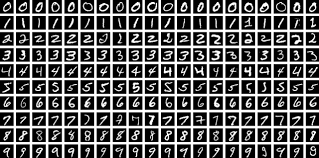
\includegraphics{img/introduction/mnist.png}
    \caption{Sample images from the MNIST dataset}
  \end{center}
\end{figure}

  \section{Literature Review}
  The MNIST dataset has long served as a benchmark for evaluating machine learning algorithms, 
especially for image classification tasks. Early approaches to MNIST relied on traditional machine 
learning methods like k-Nearest Neighbors (k-NN), Support Vector Machines (SVMs), and Logistic 
Regression, which used manually engineered features such as pixel intensity and geometric 
properties. These methods achieved moderate accuracy (90–95\%), but their reliance on feature 
extraction limited their performance. With the rise of neural networks, Multilayer Perceptrons 
(MLPs) outperformed traditional models but struggled with high-dimensional data. This led to the 
development of Convolutional Neural Networks (CNNs), which excel in capturing spatial hierarchies 
in images and have achieved exceptional performance on MNIST, consistently surpassing 99\% 
accuracy \cite{LeCun1998}.

CNNs revolutionized image recognition by automating feature extraction and improving 
generalization. The LeNet-5 architecture was one of the first CNN models for digit recognition, 
achieving significant improvements over traditional methods \cite{LeCun1998}. Further 
advancements, such as AlexNet, demonstrated the power of deeper architectures and GPU acceleration 
\cite{Krizhevsky2012}. Additionally, regularization techniques like data augmentation, dropout, 
and early stopping have been explored to enhance CNN performance and prevent overfitting. Yahia 
Assiri’s work combined these techniques, achieving state-of-the-art results on MNIST and other 
datasets like SVHN and STL10 \cite{Assiri2020}. A variation of these techniques is applied in this 
report to improve the model's performance.

  \section{Methodology}
  \subsection{Dataset Information}

The key characteristics of the MNIST dataset are summarized in \autoref{t:mnist}.

\begin{table}[H]
  \centering
  \begin{tblr}{
      hlines, vlines,
      cells = {c},
      column{1} = {l},
      cell{1}{1} = {c},
      row{1} = {bg=lightgray!100},
    }
    \textbf{Attribute}  & \textbf{Description} \\
    Number of Samples   & 70,000 \\
    Training Set        & 60,000 images \\
    Testing Set         & 10,000 images \\
    Image Size          & 28x28 pixels \\
    Channels            & 1 (grayscale) \\
    Classes             & 10 (digits 0-9) \\
  \end{tblr}
  \caption{MNIST Attributes}
  \label{t:mnist}
\end{table}

\subsection{Preprocessing}

To prepare the data for training, the following preprocessing steps were applied:

\begin{enumerate}
  \item 
    \textbf{Data Augmentation}: To increase the dataset size and improve model generalization, data augmentation 
    techniques were employed, including random rotations, shifts, and zooms.
  \item 
    \textbf{Reshaping}: Each image was reshaped to include a single channel (28x28x1) to conform to the input 
    requirements of the CNN.
  \item 
    \textbf{Normalization}: The pixel values of the images, initially ranging from 0 to 255, were scaled to a 
    range of 0 to 1 to improve the convergence of the model.
\end{enumerate}

\begin{minted}[
  frame=lines,
  baselinestretch=1.2,
  linenos
]
{python}
transform = transforms.Compose([
    transforms.RandomRotation(10),  # Rotation
    transforms.RandomAffine(0, shear=10),  # Shearing
    transforms.RandomAffine(0, translate=(0.1, 0.1)),  # Shifting up and down
    transforms.RandomResizedCrop(28, scale=(0.8, 1.0)),  # Zooming
    transforms.Resize((28, 28)),  # Rescale
    transforms.ToTensor(),
    transforms.Normalize((0.1307,), (0.3081,))  # Normalize with MNIST mean and std
])
\end{minted}

\subsection{Model Architecture}

\begin{itemize}
  \item \textbf{Input Layer}: Accepts input images of size 28x28x1.
  \item \textbf{Convolutional Layers}: Extract spatial features using filters with kernel sizes of 3x3.
    \begin{itemize}
      \item First convolutional layer: 16 filters.
      \item Second convolutional layer: 32 filters, ReLU activation.
    \end{itemize}
  \item 
    \textbf{Pooling Layer}: A max pooling operation with a 2x2 window is applied after each convolutional layer 
    to reduce spatial dimensions and computational complexity.
  \item 
    \textbf{Flatten Layer}: Converts the 2D feature maps into a 1D vector to feed into the fully connected layers.
  \item \textbf{Fully Connected Layers}
    \begin{itemize}
      \item First dense layer: 128 neurons with ReLU activation.
      \item 
        Output layer: 10 neurons (one for each digit class) with softmax activation for probability distribution.
    \end{itemize}
  \item 
    \textbf{Dropout Layer}: A dropout regularization layer with a rate of 0.8 is applied after the first dense 
    layer to prevent overfitting.
\end{itemize}


\begin{figure}[H]
  \begin{center}
    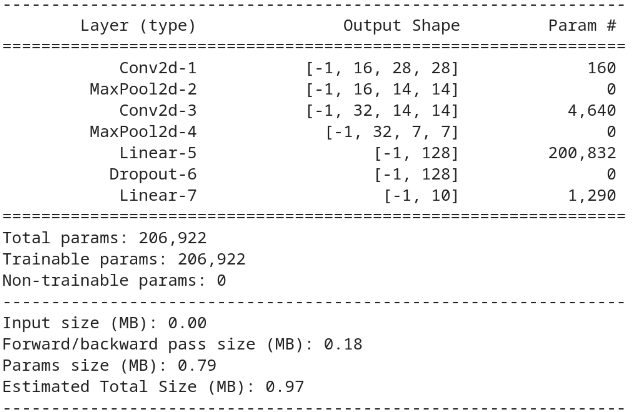
\includegraphics[width=0.7\textwidth]{img/methodology/model_summary.png}
    \caption{Model summary}
    \label{f:model_summary}
  \end{center}
\end{figure}

\autoref{f:model_summary} presents the output of the \texttt{summary} function from the Torchinfo package.

\subsection{Model Training}

The model was trained using the following configuration in \autoref{t:train_config}:

\begin{table}[H]
  \centering
  \begin{tblr}{
      hlines, vlines,
      cells = {c},
      column{1} = {l},
      cell{1}{1} = {c},
      row{1} = {bg=lightgray!100},
    }
    \textbf{Parameter}  & \textbf{Value} \\
    Loss Function       & Categorical cross-entropy \\
    Optimizer           & Adam optimizer with a learning rate of 0.001\\
    Batch Size          & 128 \\
    Number of Epochs    & 20 \\
  \end{tblr}
  \caption{Model Training Parameters}
  \label{t:train_config}
\end{table}

  \section{Results}
  The model achieve a training accuracy of 99.29\% and a validation accuracy of 99.31\%. \autoref{f:accuracy_plot} 
and \autoref{f:loss_plot} display the performance of the model during training. A confusion matrix analysis 
revealed that the model performed well across all digit classes, with most misclassifications occurring between 
visually similar digits. 

\begin{figure}
  \begin{center}
    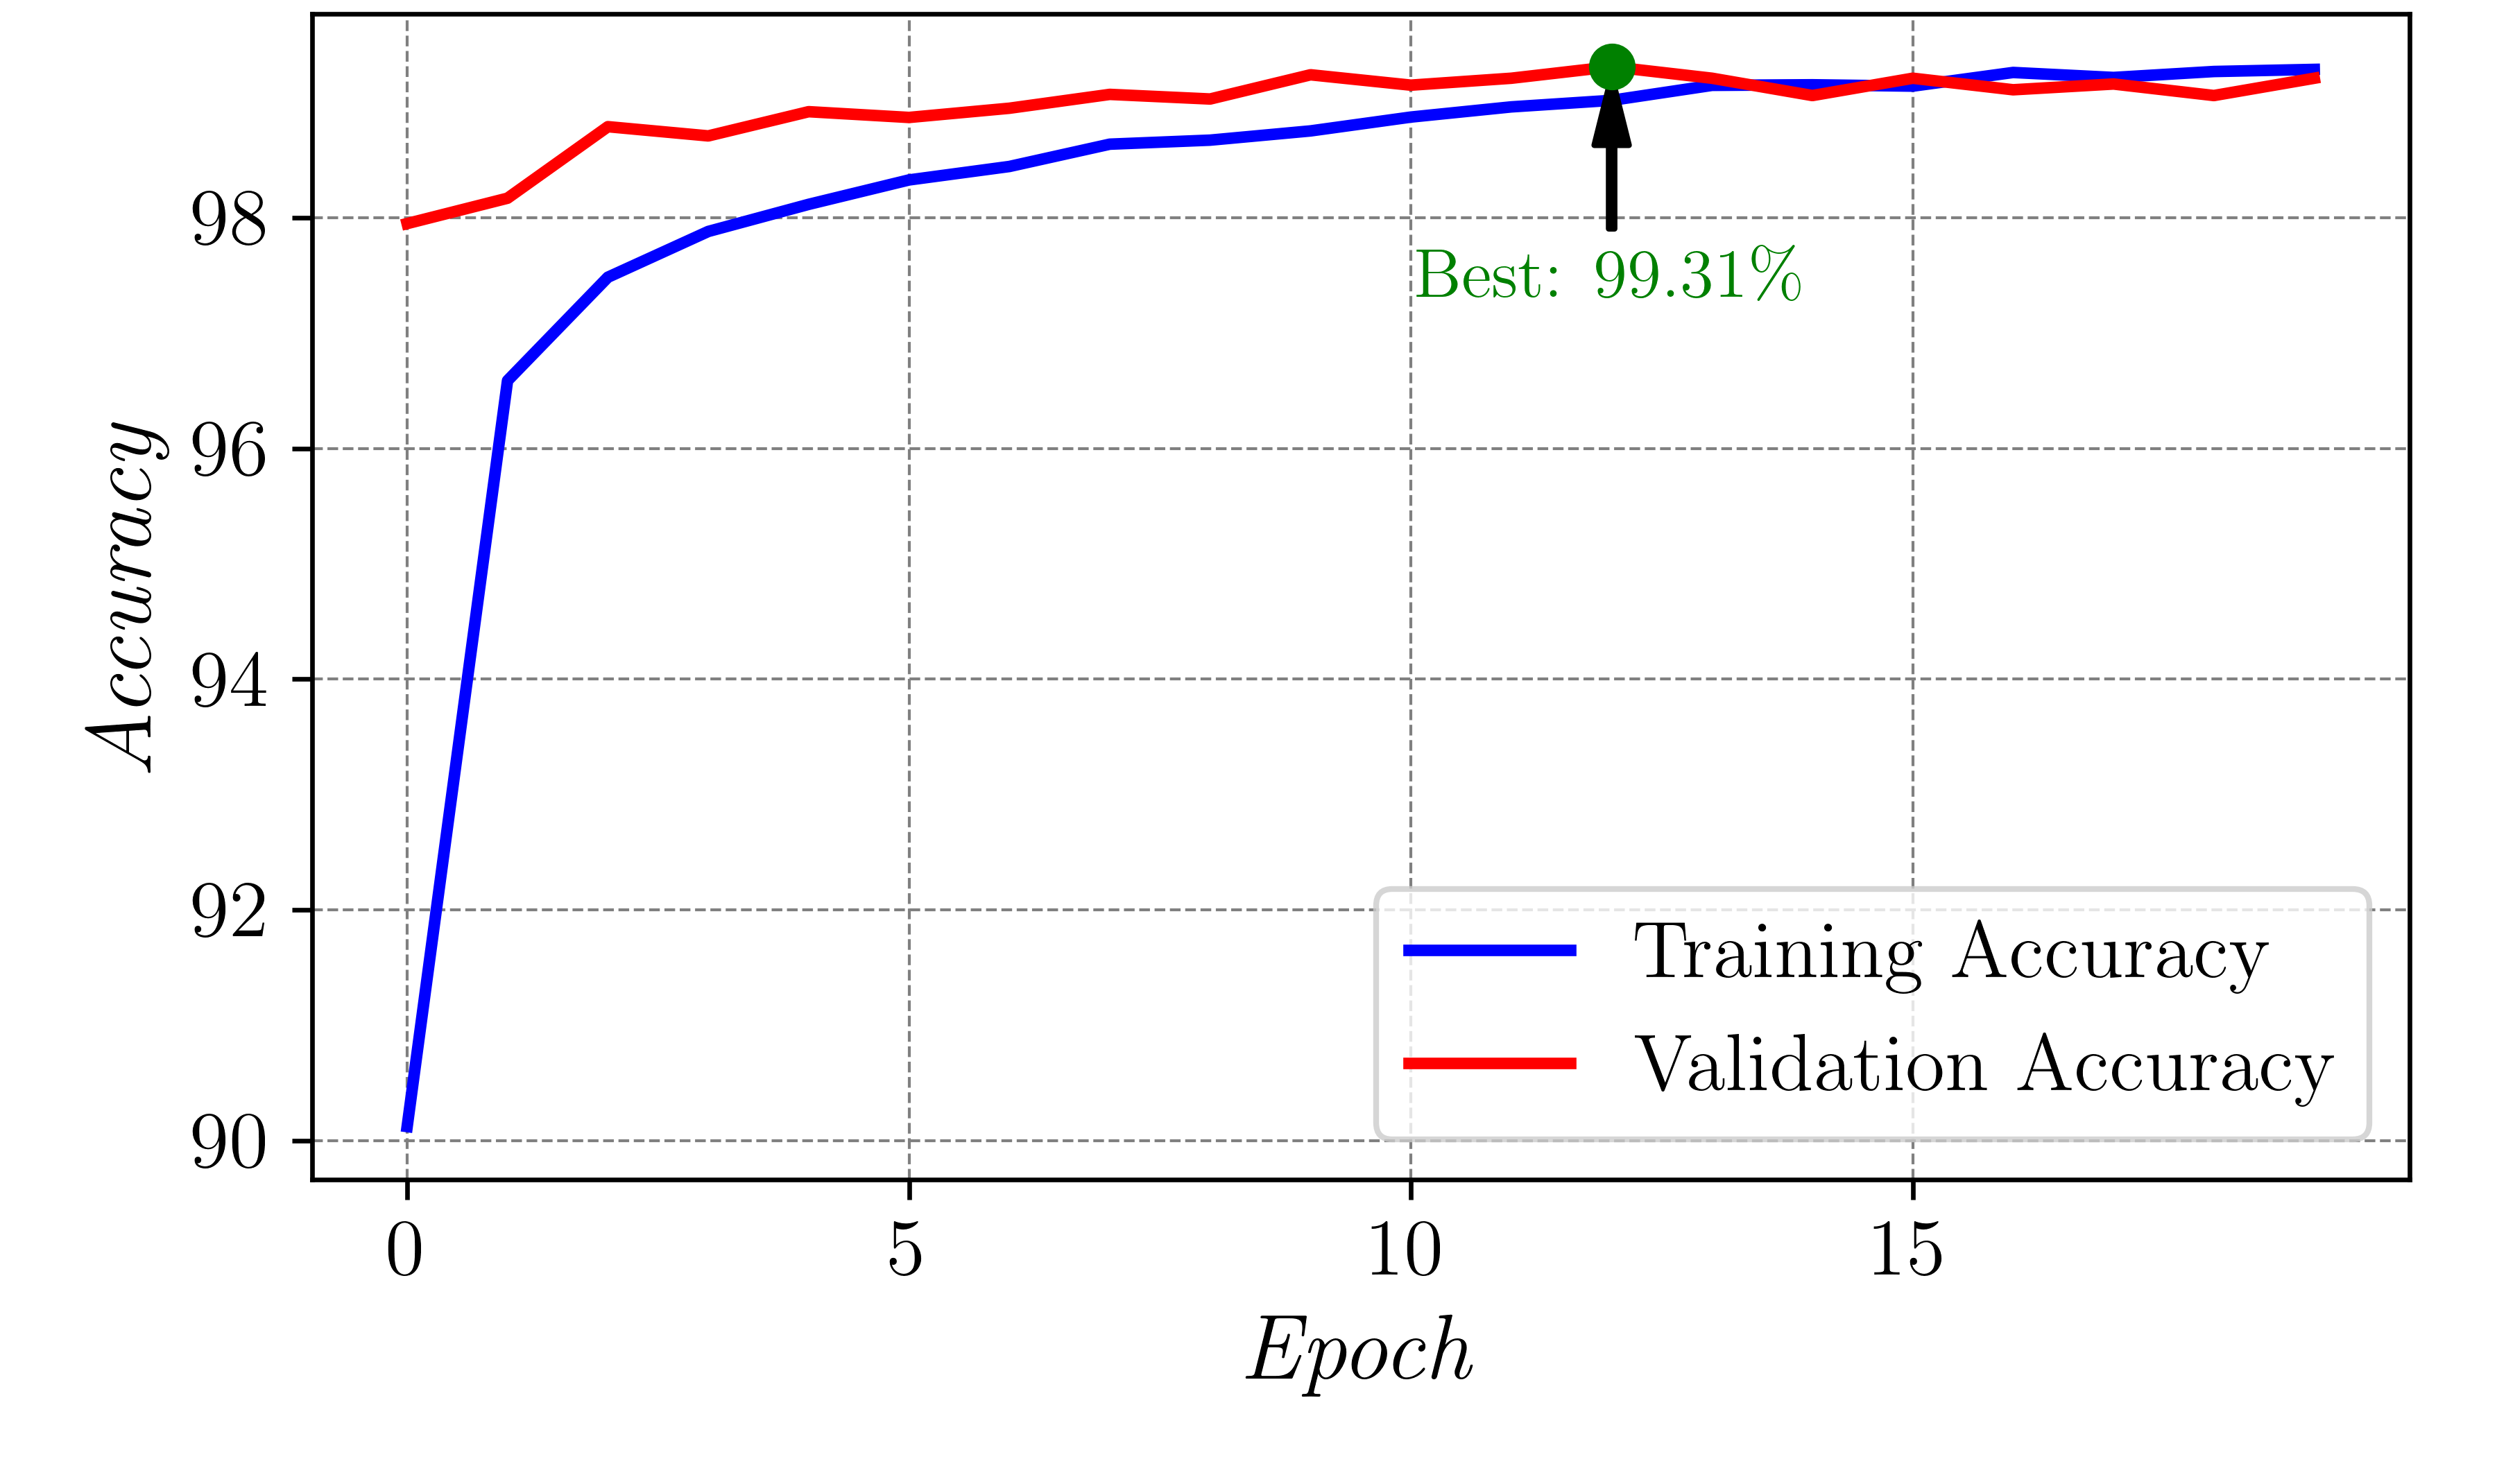
\includegraphics[width=0.7\textwidth]{img/result/accuracy_plot.png}
    \caption{Accuracy over epochs for training and validation}
    \label{f:accuracy_plot}
  \end{center}
\end{figure}

\begin{figure}
  \begin{center}
    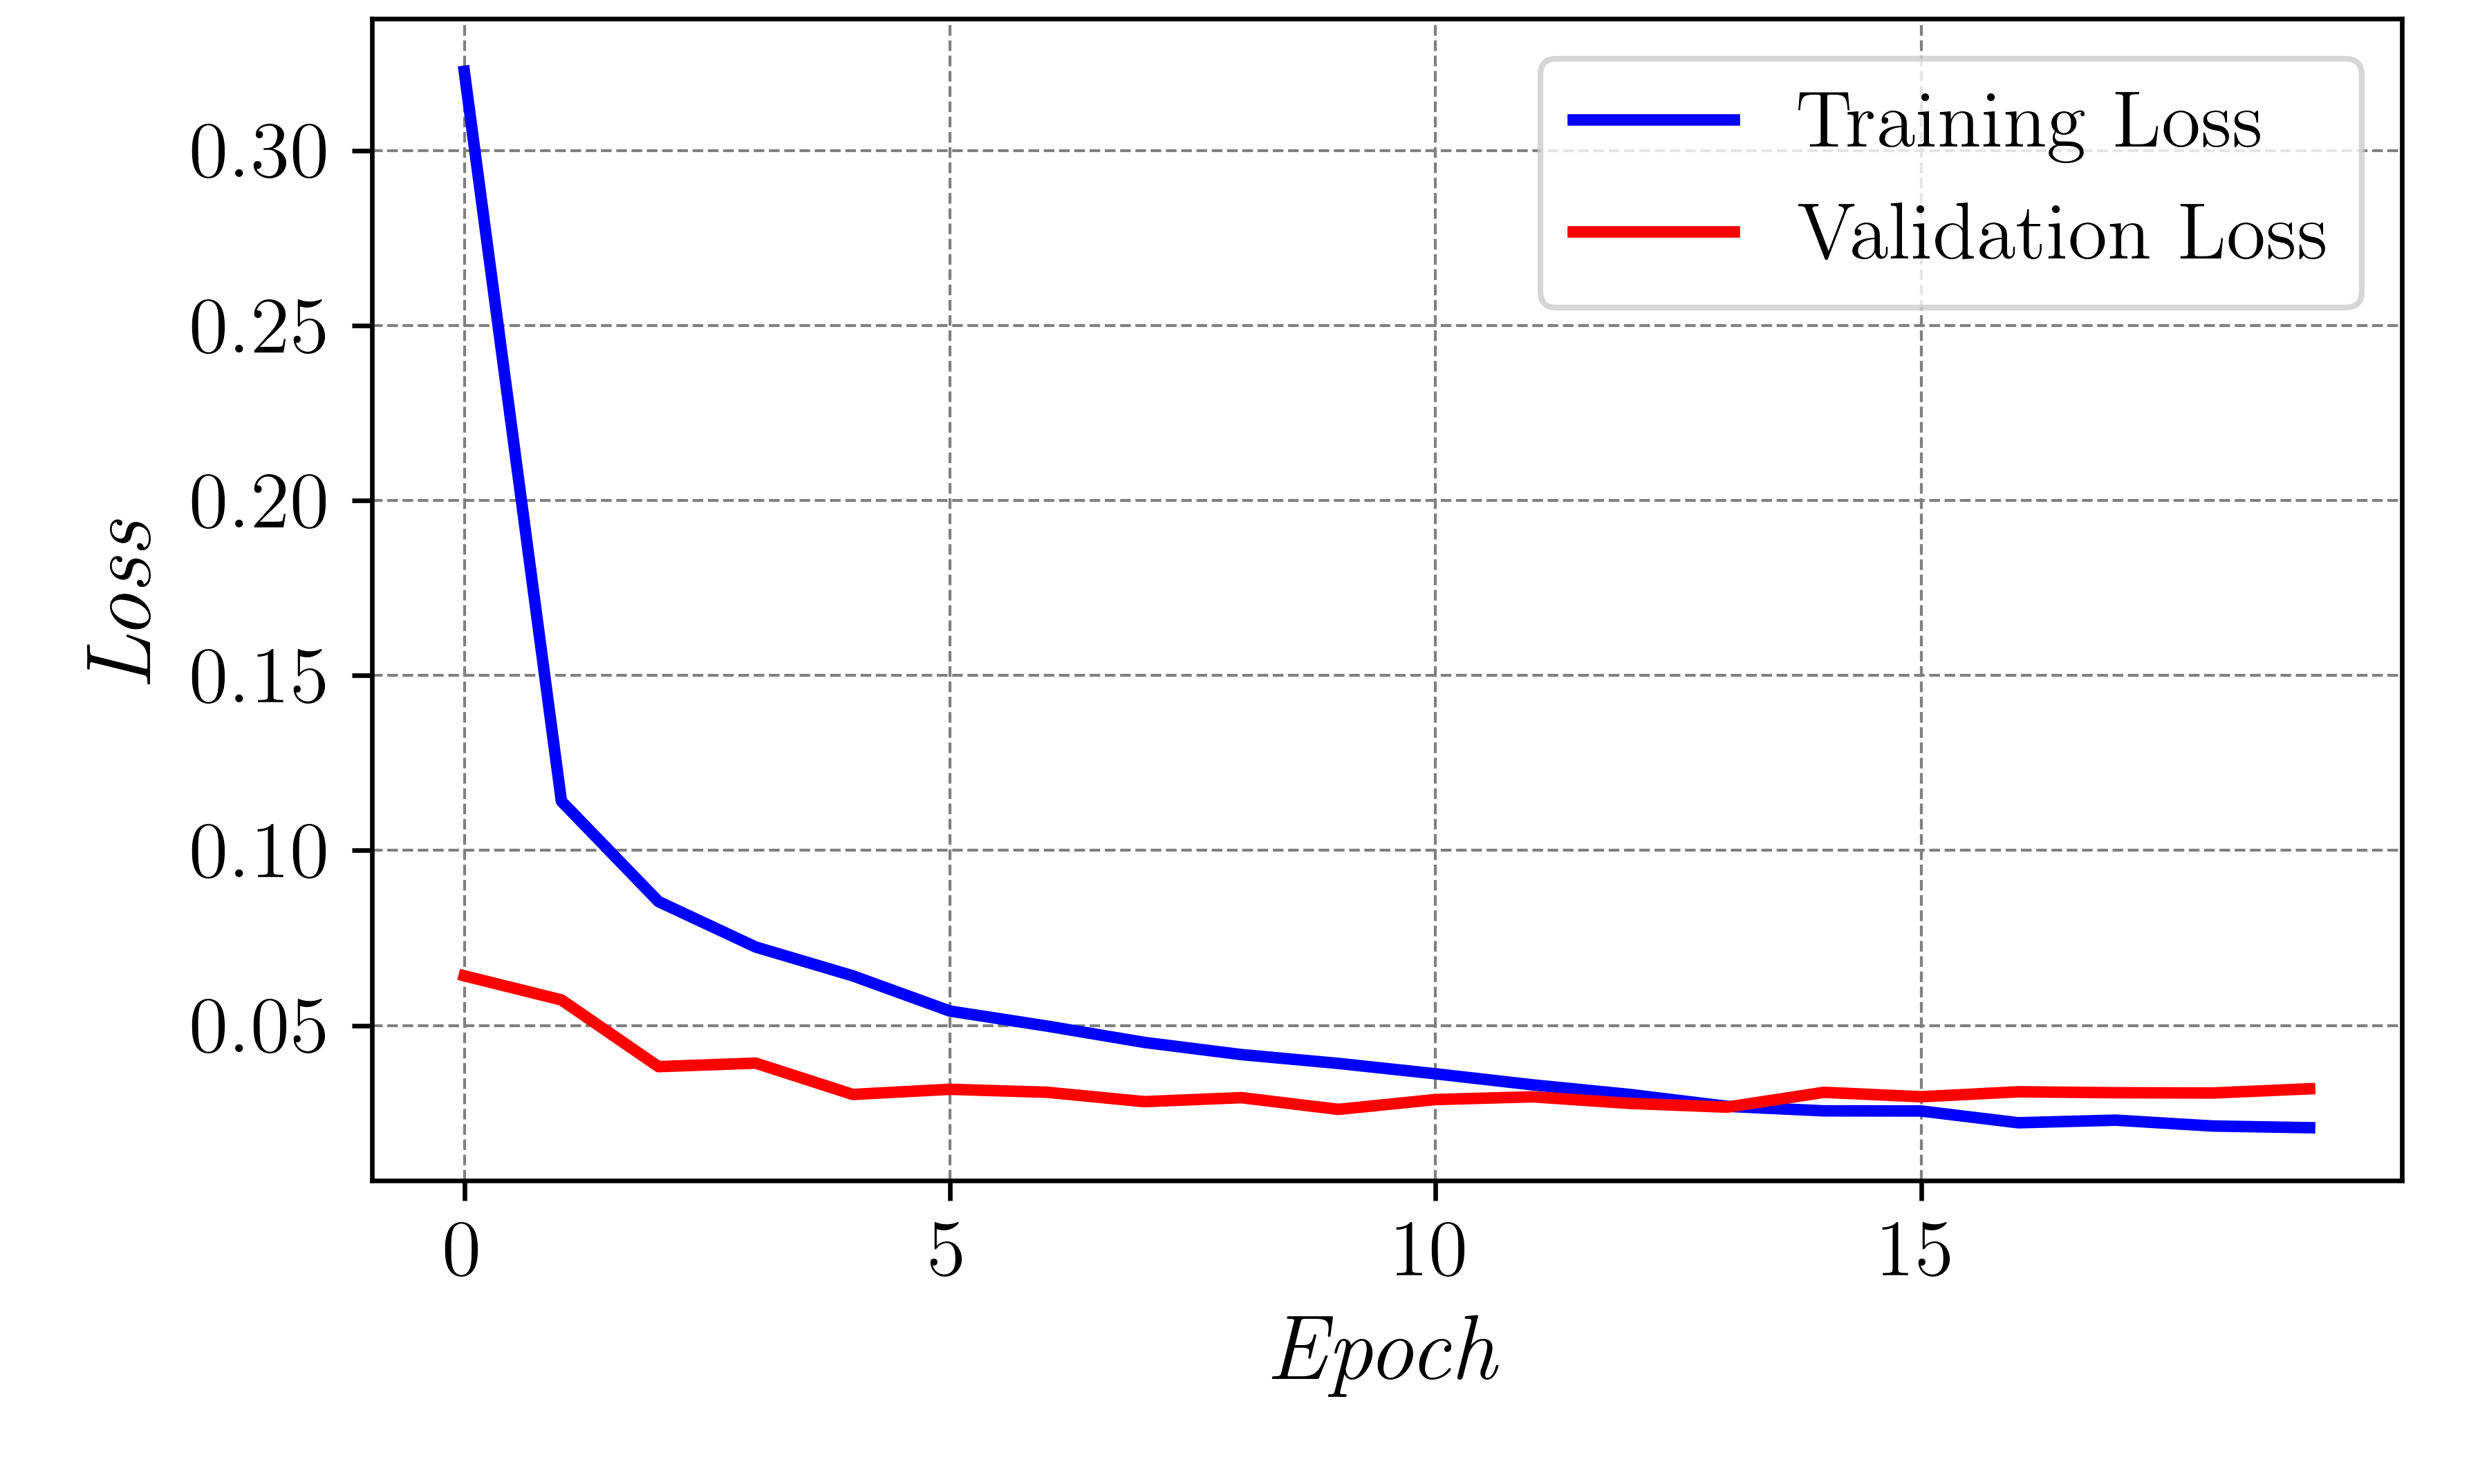
\includegraphics[width=0.7\textwidth]{img/result/loss_plot.png}
    \caption{Loss over epochs for training and validation}
    \label{f:loss_plot}
  \end{center}
\end{figure}

\begin{table}
  \centering
  \begin{tblr}{
      hlines, vlines,
      cells = {c},
      columns = {20pt},
      row{1} = {bg=lightgray!100},
      column{1} = {bg=lightgray!100,wd=48pt},
    }
    \diagbox{Pred}{True} & 0 & 1 & 2 & 3 & 4 & 5 & 6 & 7 & 8 & 9 \\
    0 & 972 & 1 & 2 & 0 & 0 & 0 & 2 & 0 & 2 & 1 \\
    1 & 0 & 1128 & 2 & 1 & 1 & 0 & 2 & 1 & 0 & 0 \\
    2 & 1 & 8 & 1013 & 3 & 0 & 0 & 0 & 5 & 2 & 0 \\
    3 & 0 & 0 & 1 & 999 & 0 & 5 & 0 & 3 & 1 & 1 \\
    4 & 0 & 0 & 0 & 0 & 973 & 0 & 2 & 2 & 1 & 4 \\
    5 & 4 & 0 & 0 & 11 & 0 & 874 & 2 & 0 & 0 & 1 \\
    6 & 3 & 2 & 0 & 0 & 2 & 7 & 941 & 0 & 3 & 0 \\
    7 & 0 & 4 & 1 & 1 & 2 & 0 & 0 & 1016 & 1 & 3 \\
    8 & 5 & 1 & 3 & 3 & 4 & 2 & 2 & 0 & 952 & 2 \\
    9 & 3 & 1 & 0 & 3 & 10 & 4 & 0 & 4 & 4 & 980 \\
  \end{tblr}
  \caption{Confusion Matrix for Model Predictions}
\end{table}

\begin{figure}
  \begin{center}
    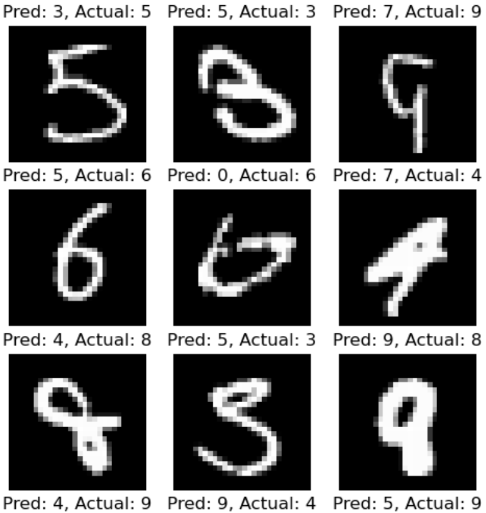
\includegraphics[width=0.4\textwidth]{img/result/wrong_samples.png}
    \caption{Examples of incorrect samples}
  \end{center}
\end{figure}

  \section{Conclusion}
  In this report, a Convolutional Neural Network (CNN) model was implemented for handwritten 
digit classification using the MNIST dataset. The model achieved high accuracy through the 
use of multiple convolutional layers, pooling, dropout, and fully connected layers. The 
performance of the CNN was demonstrated to be superior to earlier machine learning 
methods, such as k-NN and SVM, which relied on manually extracted features.

A variation of regularization techniques, including data augmentation, dropout, and early 
stopping, was applied to improve the model's generalization ability and prevent 
overfitting. These techniques have been shown to enhance CNN performance on similar image 
classification tasks. The results of this study confirm the effectiveness of CNNs for image 
classification and highlight the importance of regularization methods in achieving optimal 
performance. Future work could involve exploring more advanced CNN architectures or 
applying the model to other image datasets to further assess its robustness and scalability.


  \newpage
  \bibliographystyle{IEEEtran}
  \bibliography{references}
\end{document}
